\subsection{Specifications and Requirements}
This project idea requires the integration of power, systems, computer, optical, and web engineering to achieve a final product of a self-sustaining plant bed. The design in \autoref{fig:overall-block} shows four different subsystems the team has designated as power, control, sensing, and web.

\paragraph{Control}
The control subsystem is the brains of the entire operation. This subsystem has to accomplish four distinct tasks:
\begin{enumerate}
    \item Actuate mechanical components (linear rail, solenoid valve)
    \item Convert analog sensor data to digital data
    \item Send plant bed telemetry to web subsystem
    \item Receive commands from web subsystem and modify system accordingly
\end{enumerate}
In order to accomplish the first task, the chosen microcontroller (MCU) must be capable of driving the currents for these components and also support pulse-width modulation (PWM) for interacting with the motor controller. The second task requires that the MCU have an analog-to-digital converter. The third and fourth tasks necessitate WiFi connectivity as well as firmware support for either HTTP requests or WebSockets. These requirements for the control subsystem weigh heavily in the discussion of which MCU to choose found in Section \ref{sec:ps-control}.
\paragraph{Power}
The power system's function is self-explanatory, supply power to the entire system. This will be accomplished in two ways. First, using a DC barrel-plug to the wall, the system could be powered this way. The second way, is via the solar panels, batteries, and charge controller. Both manners of supplying power to the system must be regulated. Discussed in Section \ref{sec:ps-power} are the different ways that the charge controller can efficiently switch between battery power and the panels to increase battery health and charge level.
\paragraph{Sensing}
\paragraph{Web}
The web component of this project accomplishes three things; data analysis, reporting, and user specified control of components. The data analysis is occurring on the web because of the greater availability of compute power and greater ease of programmability. For reporting, the web will use databases to store data ad infinitum and serve this data in the form of graphs or ``live'' metrics. The web component also will be able to take a user's input to send commands back to the control system to actuate different parts such as the solenoids or to ask for a more recent data reading.
\subsubsection{Engineering Specifications}
From an engineering perspective \autoref{table:eng-specs} lays out the various metrics used to develop and design our project. 
\begin{table}[H]
    \caption{Engineering Specifications}
    \centering
    \begin{tabular}{c|c|c}
        \hline
        \textbf{Subsystem} & \textbf{Metric} & \textbf{Specification} \\\cline{2-3}
        \hline
        \multirow{8}{*}{\textbf{Control}} & Input voltage & 2.8-5.5 V \\ \cline{2-3}
                                        & Power consumption & $\leq$1.50W nominal power draw \\ \cline{2-3}
                                        & Shutdown power draw   & $\leq$100 uW \\ \cline{2-3}
                                        & Processor speed       & $\geq$20 MHz \\ \cline{2-3}
                                        & ADC resolution        & $\geq$8-bit \\ \cline{2-3}
                                        & ADC sampling rate     & $\geq$1 ksps \\ \cline{2-3}
                                        & Transmit power        & $\geq$10 dBm \\ \cline{2-3}
                                        & Receive sensitivity   & $\geq$-50 dBm \\ \cline{2-3}
        \hline
        \multirow{3}{*}{\textbf{Power}} & Battery Life & 36 Hours \\\cline{2-3}
                                        & Charge Rate & 10A \\\cline{2-3}
                                        & Regulator Efficiency & \textgreater65\% \\\cline{2-3}
        \hline
        \multirow{3}{*}{\textbf{Sensing}} & Spectra & 400nm - 1700nm \\\cline{2-3}
                                        & Resolution & \textless10nm \\\cline{2-3}
                                        & Output voltage range & 0-1.8V \\\cline{2-3}
        \hline
        \multirow{2}{*}{\textbf{Web}} & Up-time & 95\textpm.1\% \\\cline{2-3}
                                    & Storage Capacity & \textgreater16 GB \\\cline{2-3}
        \hline
        \multirow{2}{*}{\textbf{Miscellaneous}} & Dimensions & 1 m\textsuperscript{3} \\\cline{2-3}
                                                & Weight\tablefootnote{The weight of the system includes a full soil load} & \textless 50lb \\
        \hline
    \end{tabular}
    \label{table:eng-specs}
\end{table}
\begin{figure}[H]
    \caption{Overall block diagram}
    \centering
    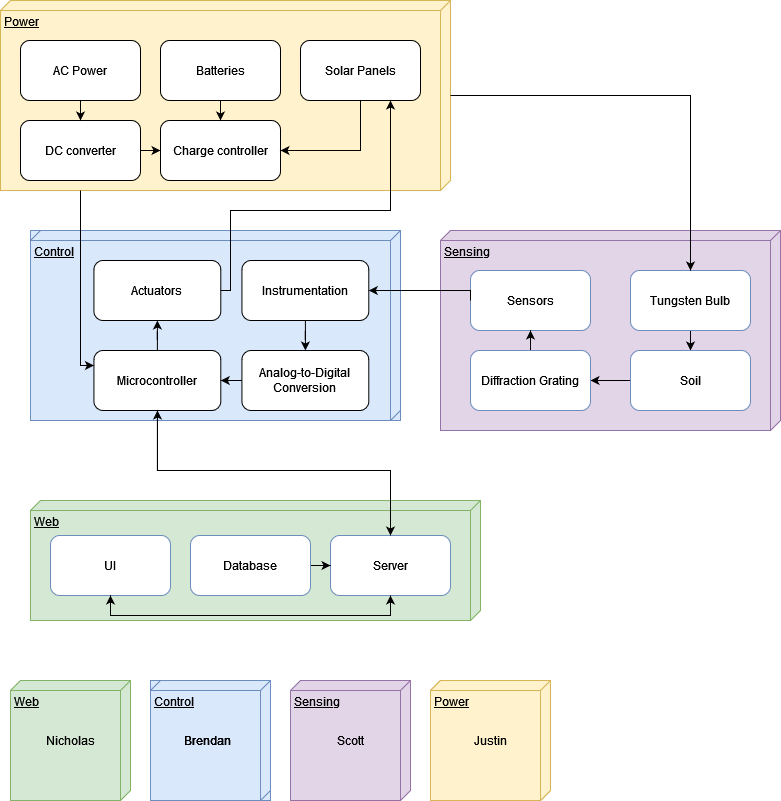
\includegraphics[width=\textwidth]{images/Overall Block Diagram.png}
    \label{fig:overall-block}
\end{figure}
\subsubsection{Marketing Requirements}
When thinking about the target market for a project like this, the team put together a list of requirements important to the consumers. The most important feature for the consumer would be how easy the product is to use and navigate. This feature ranks the highest and would be the main determining factor on whether a consumer purchases this product over a competitor. Two other highly important features to a consumer would be the accuracy of the product and the cost. The accuracy is important because it directly correlates to the success of the customer's garden. If the product is not accurate in watering the plants, the customer will be unsatisfied and the plants will not survive. Cost because every consumer has to consider their budget - how much they are willing to spend for the features they deem most important. Other customer requirements the team brought up include the durability, configurability, environmental friendliness, portability and update frequency; listed from more important to less for consumer preferences. Each of these requirements have a direct correlation to at least one of the engineering requirements set for the product. \\

The engineering requirements set by the team are: weight of the product, dimensions of the product, battery life, how much power it consumes, up-time of the website, and quality of sensor resolution. \\

When considering the customer requirement of ease of use, the team considered the impact of all the engineering requirements. Weight, battery life, and up-time all have a positive impact on customer experience. The lighter the product is, the easier it is for the customer to use because they can move it and adjust things within the product easier. The longer the batter life, the less time the consumer needs to worry when there are days with lower sunlight because the batteries can withstand a longer duration without being recharged. When the product has more up-time, the less time the consumer has to spend waiting on product updates. One of the engineering requirements that has a moderate impact on the customer experience is the sensor resolution. Although it can make a large impact on the overall product performance, its direct correlation to ease of use is not as strong as other requirements. The second most important marketing requirement listed by the team was accuracy. The only engineering requirement that had any correlation, had a strong correlation which is sensor resolution. This requirement is important to this marketing requirement because it could be a tipping point on whether a consumer purchases this product versus another. If the sensor resolution is not high enough to detect watering needs for the plant, the product will not be successful. This is why it is such an important requirement to focus on for both marketing and development of the product.\\

Something every team and every consumer is going to consider when designing or purchasing a product is the cost. The team rated this marketing requirement as an 8/10 for this product. It was not the highest priority because for a product like this, consumers will pay more to have a more accurate and easy-to-use product. The team also considered that customers using this product will do more research about the technical features because they are most likely growing fruits or vegetables that they will consume. Unfortunately, most things that increase the quality and appeal of the product, have a negative relationship that is strong in correlation. When the team looks at lighter materials, those materials increase the price. When adding a longer battery life and lowering power consumption, price will increase proportionally to how much those requirements change. To increase the resolution of the sensor, the team and consumers will have to pay more for the increase in quality and performace. The only requirement that  correlates to cost that was not strong, but still has an impact is the up-time. The more up-time of the product services, the more cost that is involved, but it is a smaller margin compared to the other requirements that directly impact the cost of the product. \\

Durability is most affected by the engineering requirements of weight and dimension. If the product materials are different, the durability will change and if the dimensions change shape or length, the construction may be different affecting product strength. Weight will have a stronger impact than durability because it is something cosumers will consider more heavily and the materials will impact more. This is why weight has a strong correlation and dimensions are moderately correlated.\\

% Notes to change: the triangles need to be updated to filled in circles. 
% Add triangles to the following: up-timeXcost, 
% Change to unfilled circles: sensorXcost,durabilityXdimensions
% Filled in Circles: DurabilityXweight





\begin{figure}[H]
    \centering
    \caption{House of Quality}
    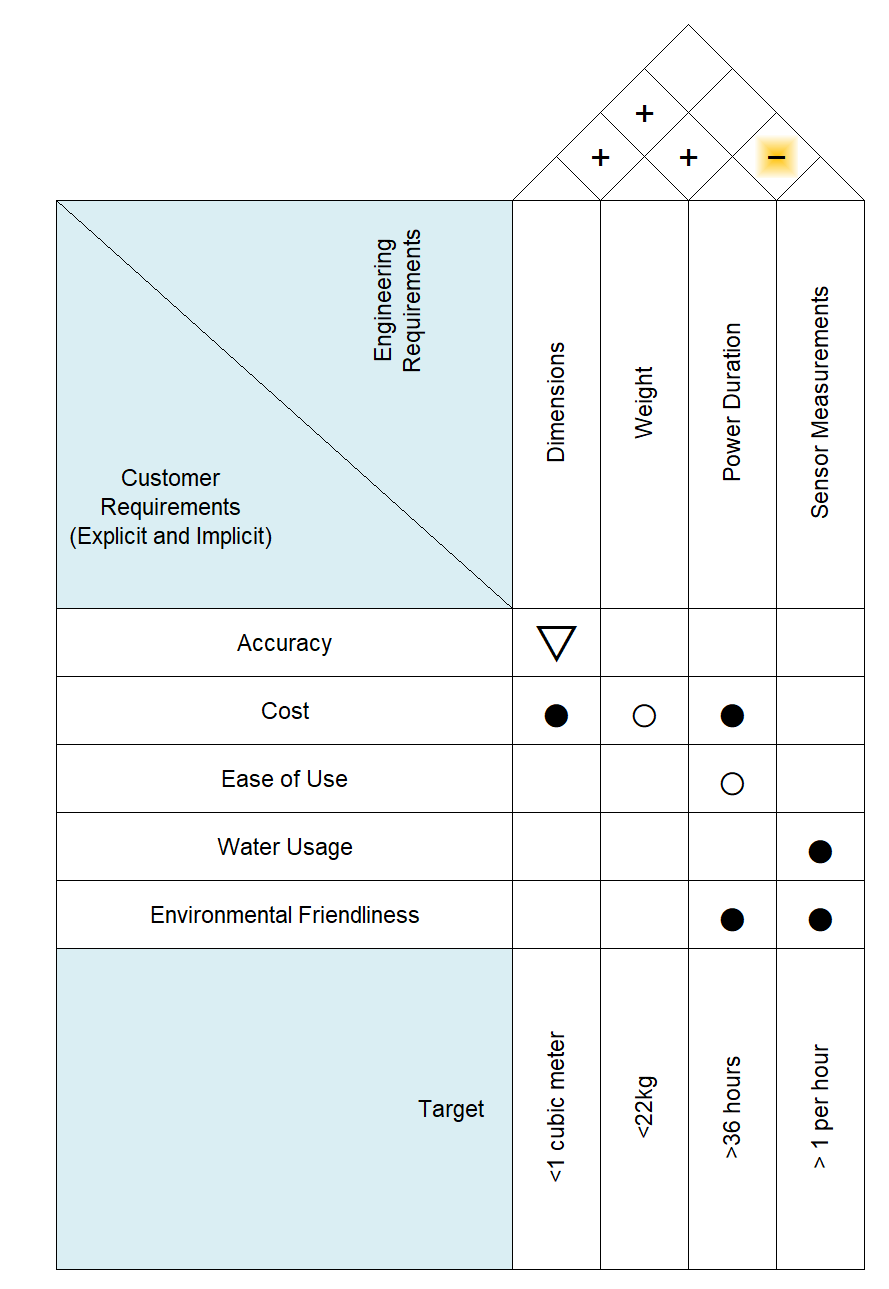
\includegraphics[width=\textwidth]{images/HouseOfQuality.PNG}
\end{figure}